

\begin{figure}
	\centering
	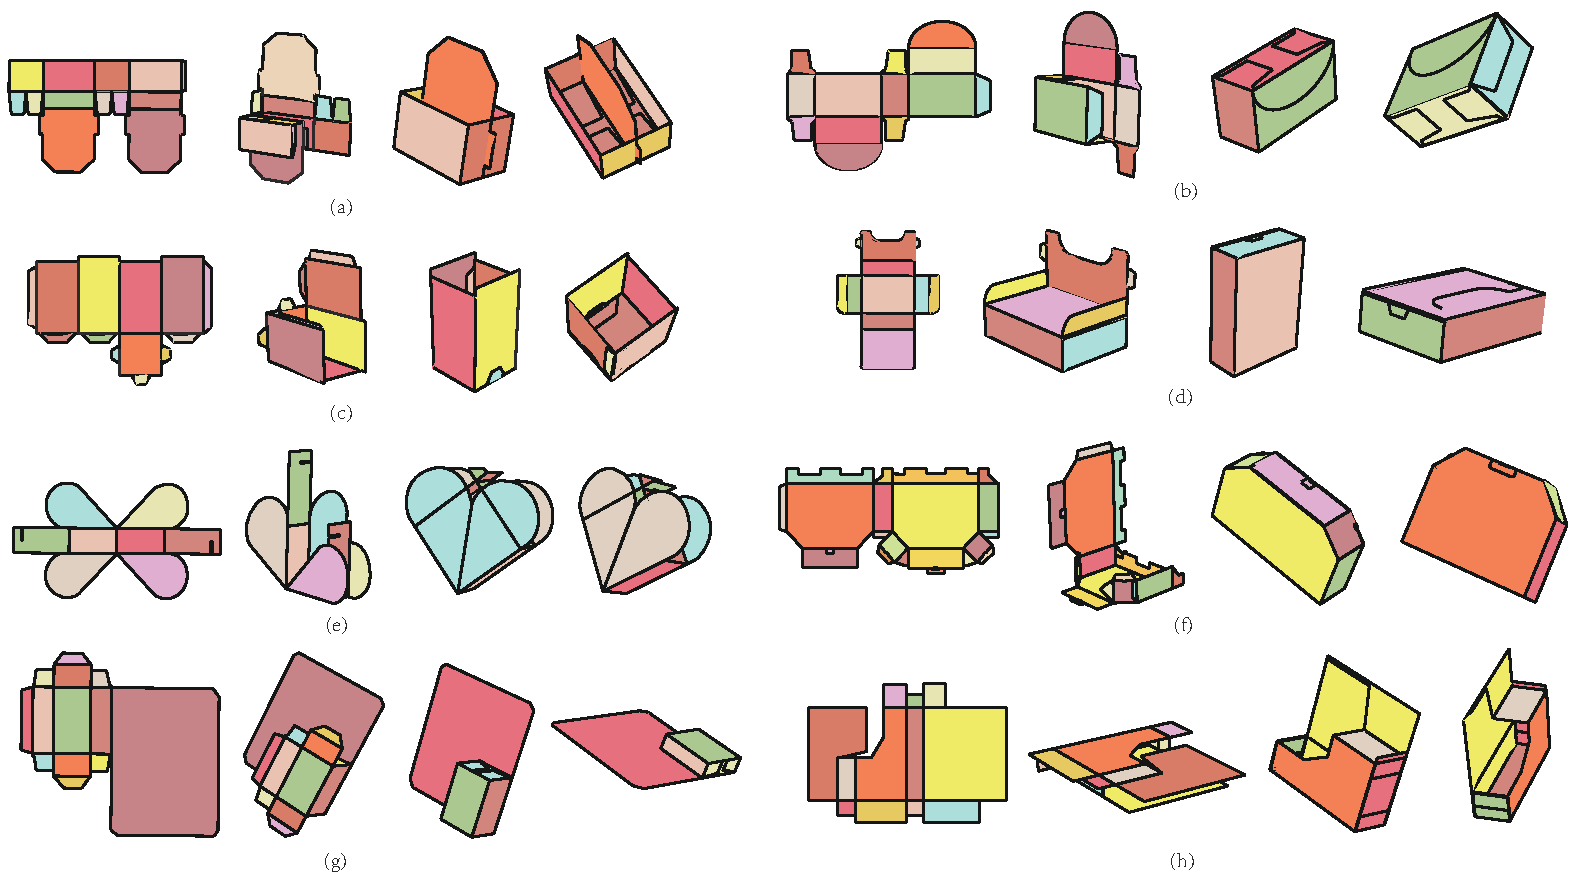
\includegraphics[width=\textwidth]{images/moreAutomatic}
	\caption{More carton examples that can be automatically generated. For each example, four subfigures are shown from left to right: the input 2D layout, an intermediate stage during folding, and the final 3D shape from two views.}  
	\label{fig:automatic-more}
	
\end{figure}

%%%%%%%%%% Results with refinement %%%%%%%%%%

\begin{figure}
	\centering
	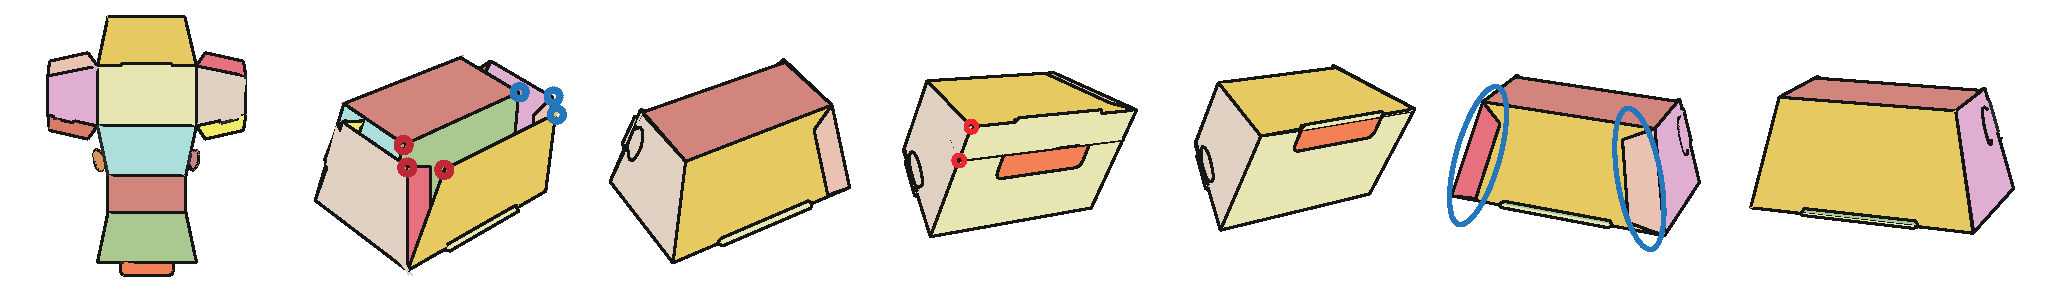
\includegraphics[width=\textwidth]{images/105}
	\caption{The complete process of generating a carton model with user interactions. From left to right: the input structural layout used to generate a flat polymesh, the initial 3D model, two vertex merging confirmations, one panel pasting, and the final 3D model.}
	\label{fig:result}
\end{figure}

\begin{figure}
	\centering
	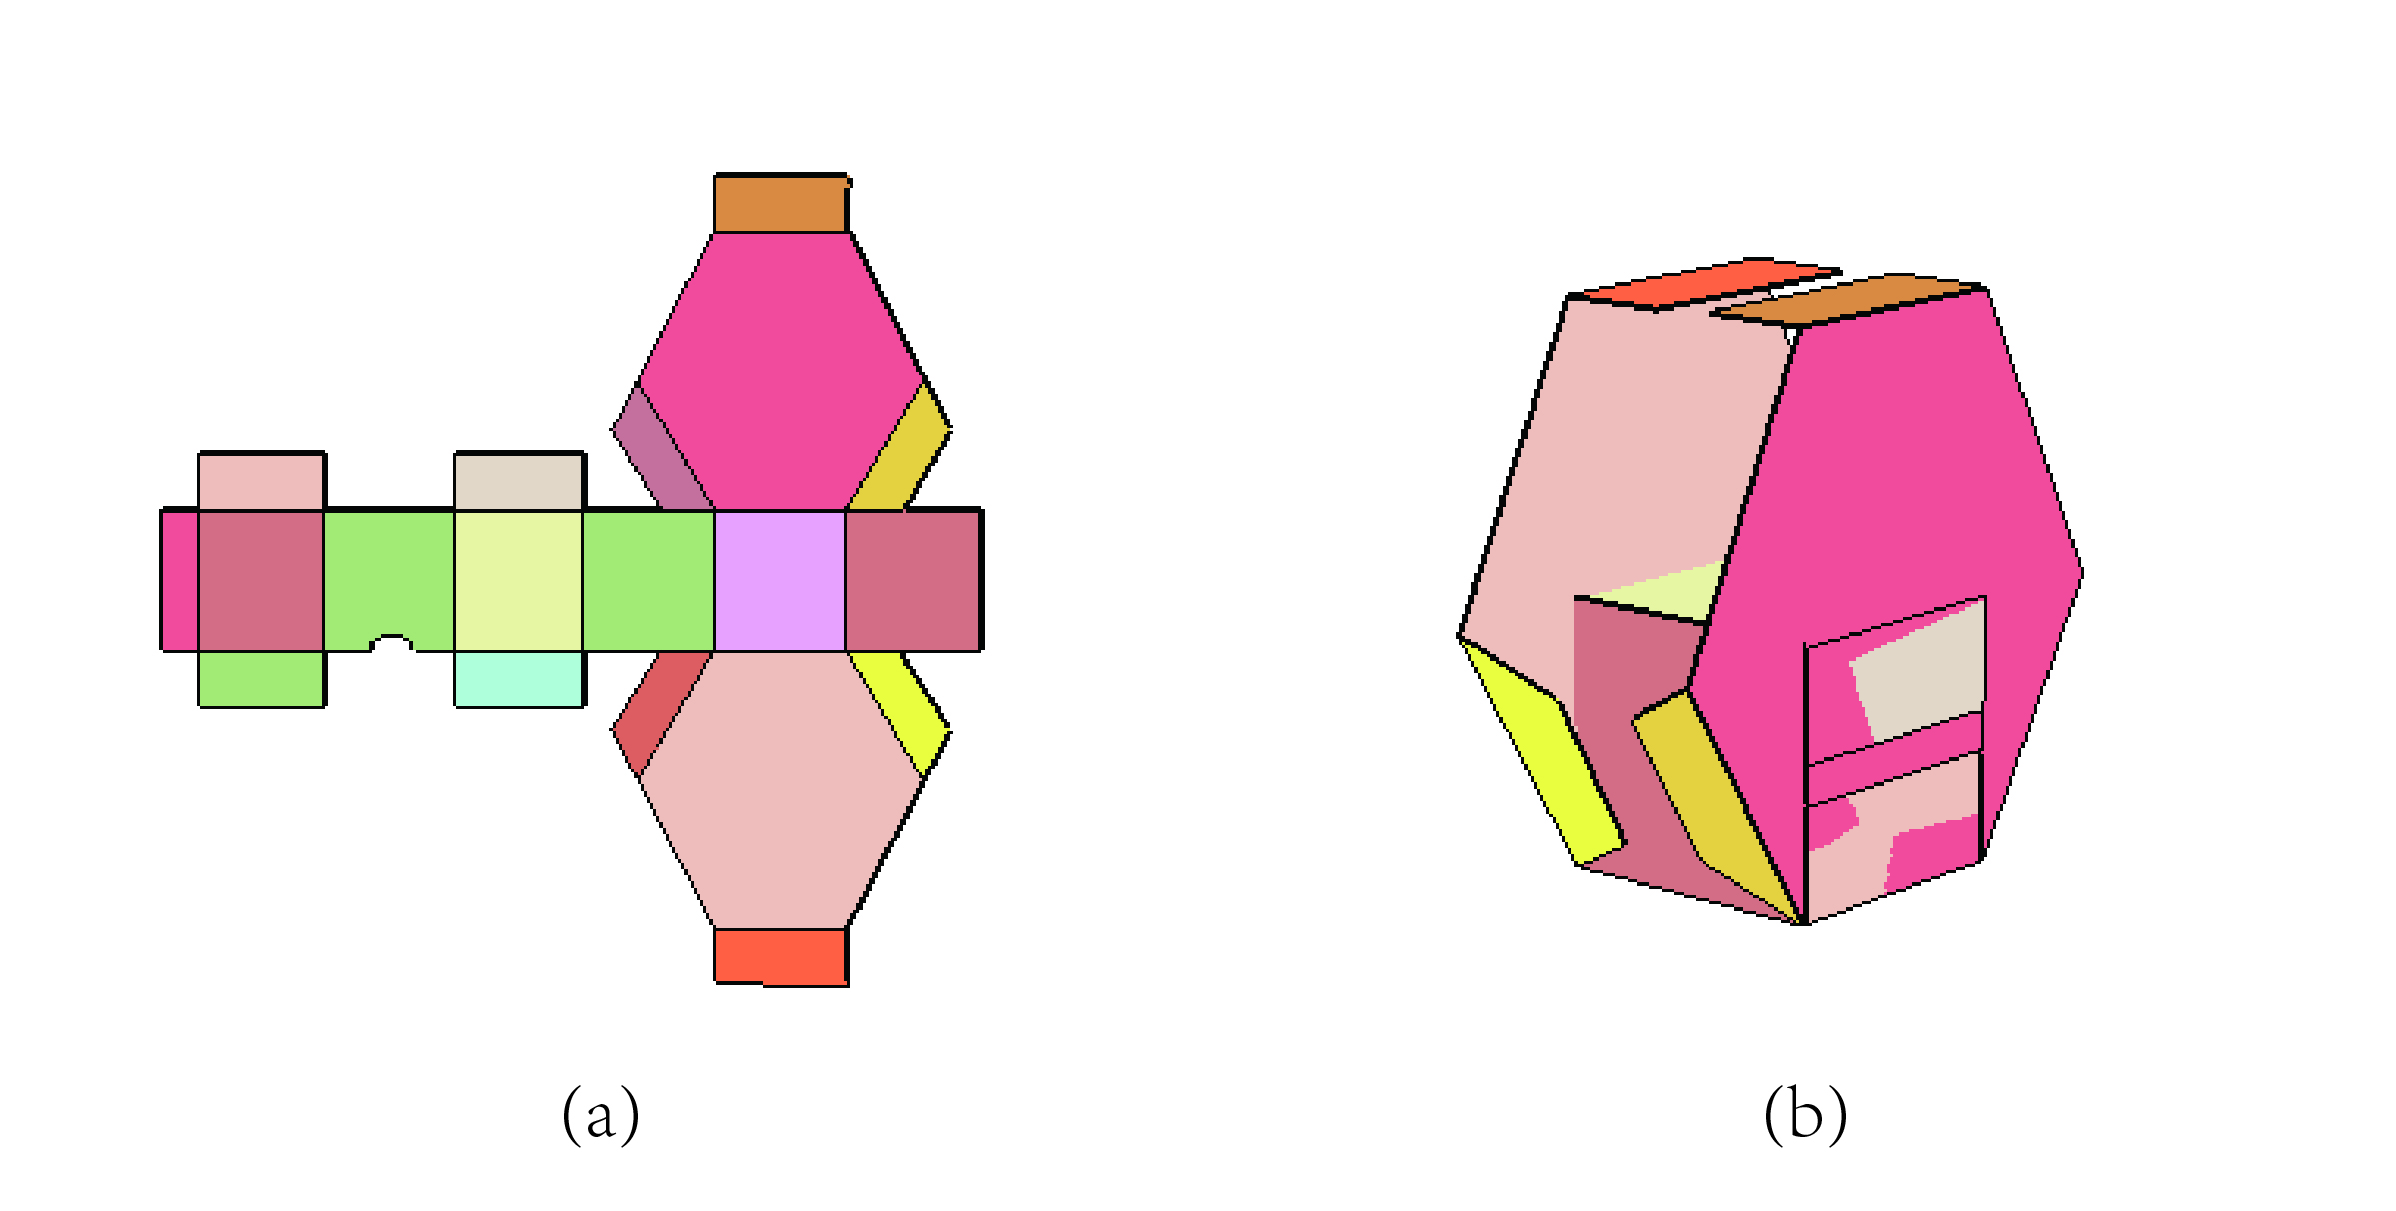
\includegraphics[width=0.9\textwidth]{images/limitation}
	\caption{When given a 2D layout (a), our system generates an initialized result (b). After nine user interactions, including selecting merging vertexes and panel pasting, the final model is obtained as (d). }
	\label{fig:hexagon}
\end{figure}

\begin{figure}[h]
	\centering
	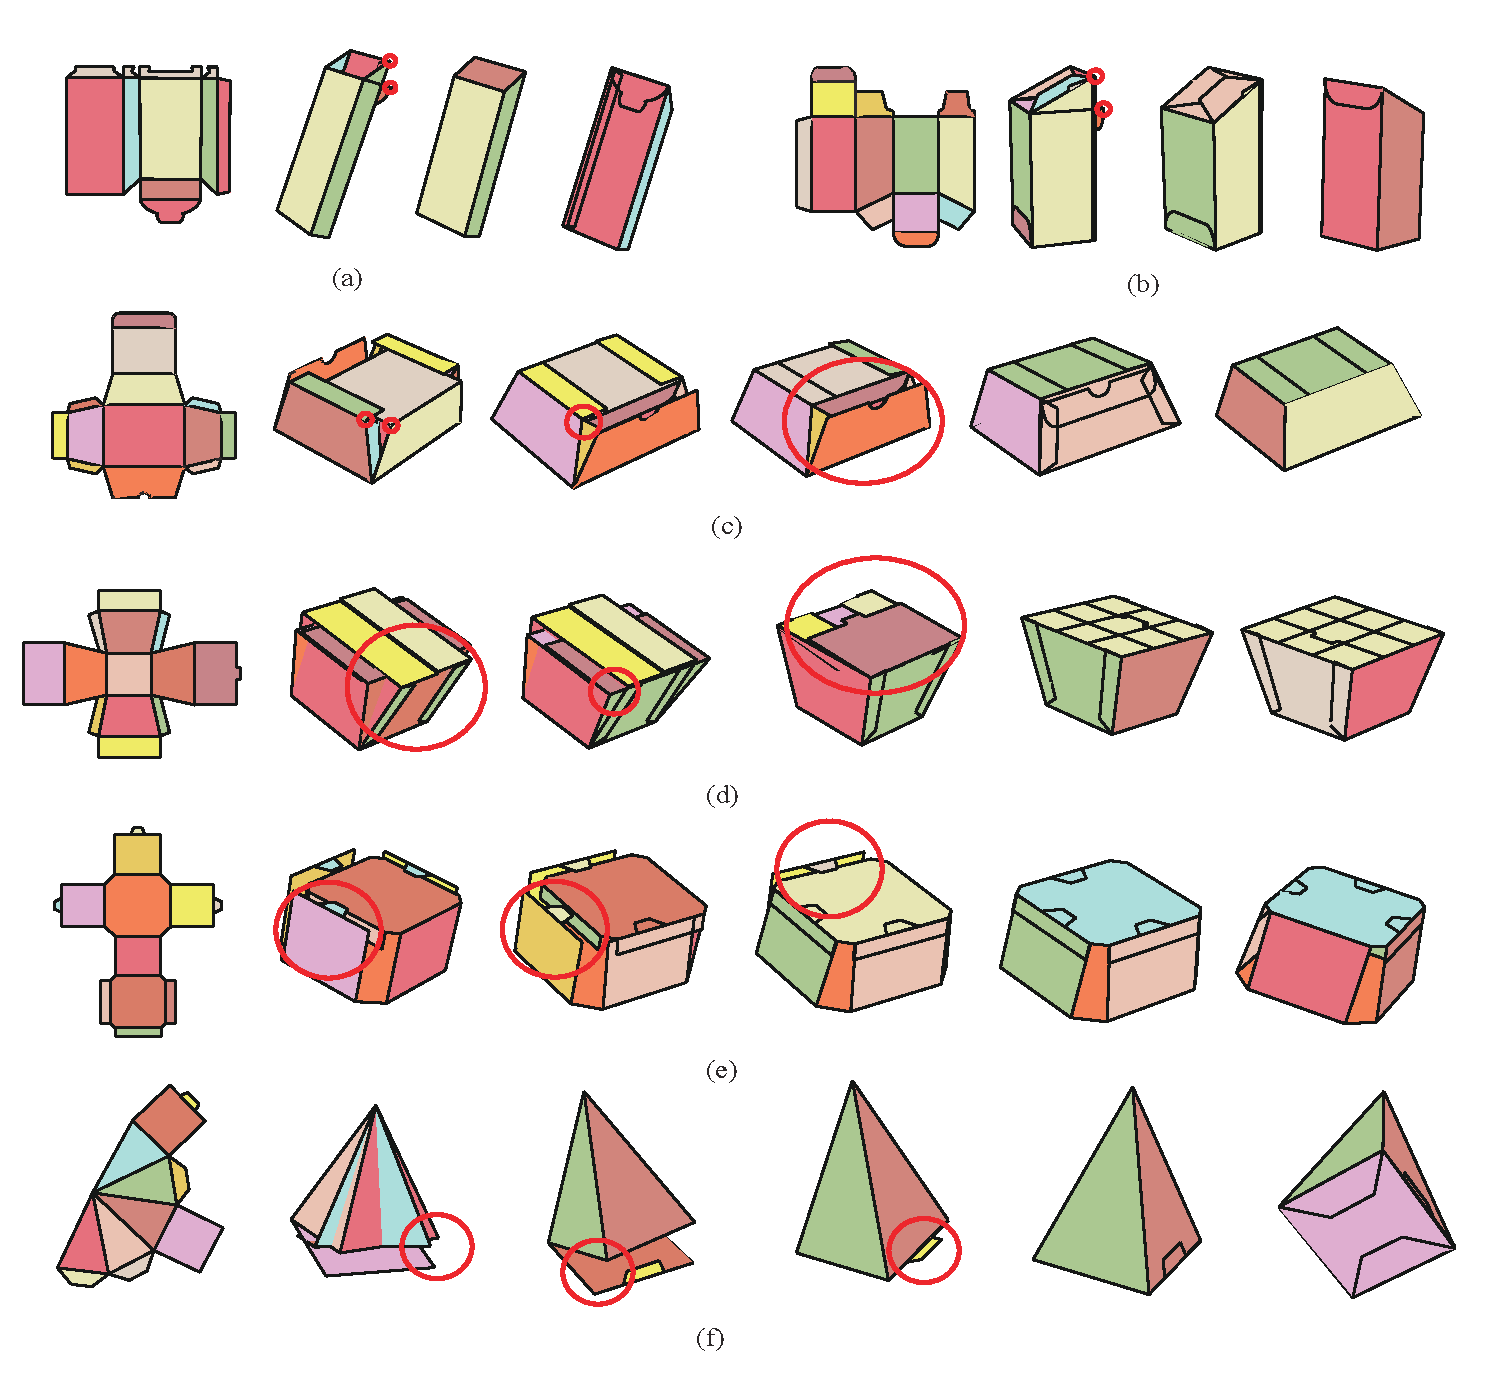
\includegraphics[width=0.9\textwidth]{images/newMore}
	\caption{More complicated results with shape refinement. In each example, the first two images represent the 2D layout and the initial model, and the last two show the final model from different views. The middle images illustrate the intermediate shapes with different shape constraints, which are marked in red circles.}
	\label{fig:result-more}
\end{figure}


\section{Results and Discussion}\label{sec:result}


Based on the two-step approach for folding a carton model, as well as the suggestive user interface, our system is natural and easy to use. 
%
We will show a series of results of cartons in various shapes. 
%
A user study was also conducted to examine the effectivenss of our suggestive system.


\subsection{Carton Results}

%%%%%%%%%%% Fully automatic results %%%%%%%%%%%

For most cuboid cartons, their 3D models can be generated by folding each edge by $\pi/2$, as shown in Figure~\ref{fig:initial-automatic} and Figure~\ref{fig:automatic-more}.
%
Nowadays, in the common design process, designers typically spend a great deal of time on manually creating 3D carton models in 3D modeling software. 
Our suggestive interface saves a significant amount of effort, so designers can focus more on designing the appearance of cartons. 


For more complicated cartons, shape refinement is required. 
The entire process of creating a carton model from a 2D layout is illustrated in Figure~\ref{fig:result}.
%
The final model is generated after a total of three clicks: two clicks to confirm vertex merging and one click to confirm panel pasting.
Note that our system automatically detects these possible geometric editing options for users to select; therefore, the user eliminate the tedious process of selecting edges or vertexes and assigning precise angles or positions to them.
%
A more challenging example is shown in Figure~\ref{fig:hexagon}. 
By initially folding each edge as $\pi/2$, our system first generates a cube inside the carton for the six square faces. 
Occasionally, our system fails to detect the mergeable vertexes with a small threshold $\epsilon$ to merge nearby vertexes; however, the user could manually merge two vertexes. Then, our system automatically detects two symmetric vertexes that also can be merged. 
%
Finally, a hexagonal carton is generated after a limited number of user interactions.
%



More carton models, which were generated using our system with a few user interactions, are shown in Figure~\ref{fig:result-more}.
The statistics of the panel number, edge number, and number of user interactions are listed in Table~\ref{table:statistics}. 
We can see that only a few user interactions are needed for a variety of shapes in order to confirm the system's suggestions.
 

\begin{table}
	\centering
	\caption{Statistics of the number of edges $N_{edge}$, number of panels $N_{panel}$, and the number of user interactions $N_{interaction}$ for the examples shown in this paper.}
	\setlength{\tabcolsep}{1pt}
	\begin{tabular}{c|c|c|c|c|c|c|c|c|c|c|c|c}
		\hline
		Examples & Fig.\ref{fig:automatic-more}(a) & Fig.\ref{fig:automatic-more}(b) &  Fig.\ref{fig:automatic-more}(c) & Fig.\ref{fig:automatic-more}(d) & Fig.\ref{fig:result} & Fig.\ref{fig:hexagon} & Fig.\ref{fig:result-more}(a) & Fig.\ref{fig:result-more}(b)& Fig.\ref{fig:result-more}(c) &  Fig.\ref{fig:result-more}(d) & Fig.\ref{fig:result-more}(e)& Fig.\ref{fig:result-more}(f)\\
		\hline
		$N_{edge}$ & 49 & 62 & 46 & 45 & 54 & 67 & 40 & 43 & 42 & 38 & 48 & 30\\
		$N_{panel}$  & 13 & 13 & 11 & 13 & 14 & 19 & 11 & 13 & 13 & 13 & 12 & 11\\
		$N_{interaction}$  & 0 & 0 & 0 & 0 & 3 & 9 & 1 & 4 & 1 & 3 & 3 & 3\\ 
		\hline
		\end{tabular}
		\label{table:statistics}
\end{table}


%%%%%%% User Study %%%%%%%%%%%%%%%%%%%%%%%%%%%%%
 
\subsection{User Study}
\label{sec:userstudy}
\section{User Study}
We conducted a user study to examine the productivity of our system to construct the corresponding 3D model of the planar layout, and the guiding effectiveness of users fabricating the practical mockup. The experiment was separated into two parts. In the first experiment, participants were asked to construct the 3D model from the same 2D layout using our system and STUDIO after a brief introduction, and a two-alternative forced choices design was designed, with participants asked to choose which system they preferred to use considering the complexity of operations or modeling time. Furthermore, participants needed to rate our system from one to five on the necessity of layout optimization, five is for very necessary. Tn the second experiment, participants were separated equally into two groups, one group was asked to fold the given practical printed paper into 3D mockup with the guide video provided by our system and the fabrication time was recorded compared with another group without the guide video. Our goal was to test the following hypotheses:

\begin{itemize}
	\item \textbf{Hypo1:} Our system need less time and effort to construct a digital 3D mockup than traditional software.
	\item \textbf{Hypo2:} Our system can provide novel and practical function to reach diverse layouts.
	\item \textbf{Hypo3:} Our system can guide the fabrication of cartons.
\end{itemize}

\subsection{Procedure}
We began the experiment with each participant by explaining the background and the instructions of our system and STUDIO. Ten layouts from thirty-four 2D design layouts were given to participants for folding, and at least three of them would need refinement. Participants were allowed to watch the final model of the layout to instruct construction. After operating the two systems. each participant was asked to answer a questionnaire including four(??five?? not clear how to use the question of modeling experiment) questions: which of two systems participants preferred based on the simplicity of operation. which of two systems participants preferred based on the modeling time, score one to five on the necessity of layout optimization in our system. and write the suggestions to our system.

\subsection{Discussion}
We consider our three hypotheses in turn. With respect to Hypo1, we collect the answers of former two questions, the result is show in Figure~\ref{fig:preference}. We also performed a pared-samples t-test at level $\alpha = 0.05$ to compare the preference significance, and the test shows our system is significant preferred by participants.(?How to show t-test result?) Considering the suggestions from participants preferring STUDIO, the operations need to be learned from STUDIO is just selecting folding lines and assigning angles, while ours provides multiple selections to construct the final model. However, when most participants think the steps need to take to final model is much less than STUDIO, which is the main reason choosing our system. Take Figure~\ref{fig:result-more}(e) for example, participants usually took much time to slightly adjust the folding angles of creases, while ours just needs three clicks.

\begin{figure}
	\centering
	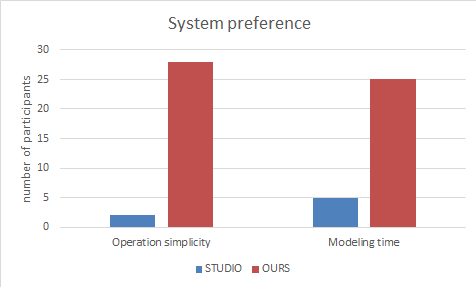
\includegraphics[width=0.4\textwidth]{images/preference.png}
	\caption{The collection of the former two answers related to the preference based on modeling time and operation simplicity. }
	\label{fig:preference}
\end{figure}

With respect to Hypo2, twenty-four participants gave the highest score to our layout optimization function. In addition to explore the diversity of 2D layouts, it also can adjust the imprecise faces on 2D layout to reach an ideal model by construction. Figure~\ref{fig:correction} shows the final model constructed by our system and STUDIO, as we can see, the side face 1 is higher than face 2 in the model constructed by STUDIO, while in our system, we can correct these design error by merging vertices circled in red.

\begin{figure}
	\centering
	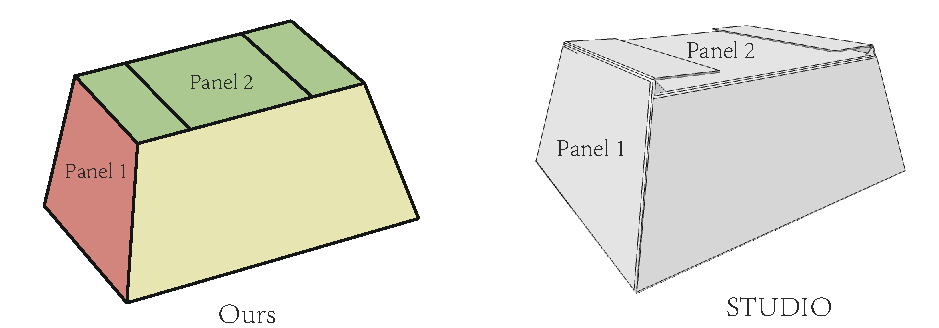
\includegraphics[width=0.5\textwidth]{images/comparison}
	\caption{Different model constructed by our system (a) and STUDIO (b). }
	\label{fig:correction}
\end{figure}

For Hypo3, XX (add t-test figure??? into Figure 13)







\paragraph{Limitations.}

\begin{figure} 
	\centering
	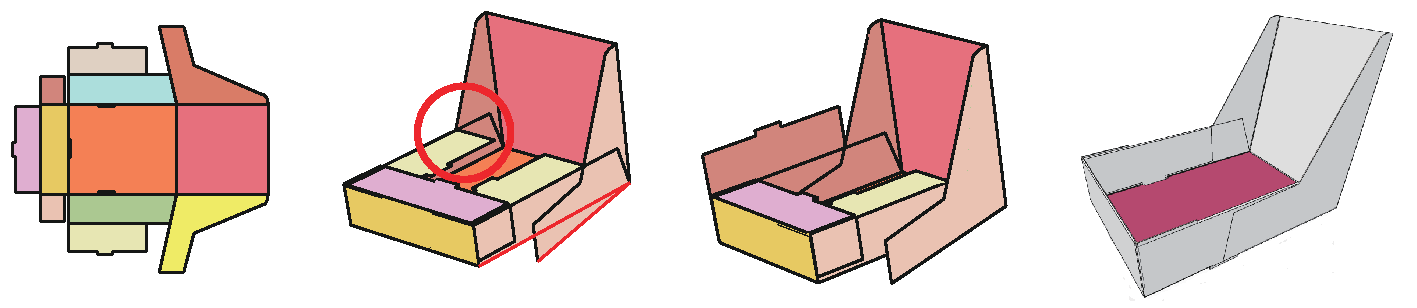
\includegraphics[width=0.8\textwidth]{images/moreLimitation}
	\caption{Limitations in our current system. From left to right: a 2D layout, the initial model after folding each edge by $\pi/2$, the optimized model after pasting the three panels circled in red, and the desired carton model constructed from the 2D layout. }
	\label{fig:failure}
\end{figure}

%%%%%%%%%% Limitations and discussions %%%%%%%%%%%%%%%%%%%%%%%%%%%%%%%%%

Our suggestive shape optimization is very useful in a wide range of cases. Nevertheless, there are still some failure cases that our system can not deal with. Figure~\ref{fig:failure} shows a case that is challenging for our current system. The panels circled in red should be pasted together to produce a strong enforced panel.
However, our system only ensures the coplanarity of the selected three panels, and as a result, the yellow panel is expanded in the opposite direction. 
%
Moreover, the pink back panel is orthogonal to the bottom panel after initialization, and the two red edges are not aligned.   
This can be solved by adding more editing tools, such as aligning edges, or assigning a folding angle for a specific edge, such as STUDIO.

